\documentclass{article}
%%%%%%% PACKAGES %%%%%%%%
\usepackage[utf8]{inputenc}
\usepackage{graphicx}
\usepackage{geometry}
\geometry{a4paper, margin=1in}
\usepackage{hyperref}
\usepackage{titling}
\usepackage{caption}
\usepackage{subcaption}
\usepackage{float}
\hypersetup{
    colorlinks=true,
    linkcolor=blue,
    filecolor=magenta,      
    urlcolor=cyan,
}

\title{Assignment 2: Swarm Intelligence\\CS 451: Computational Intelligence}
\author{Ali Asghar Yousuf $\mid$ Muhammad Murtaza}
\date{\today}

\begin{document}

\maketitle

\section{Ant Colony Optimization}

\subsection*{\begin{center}
  Capacitated Vehicle Routing Problem
\end{center}}

Plot of the best and average solution of Capacitated Vehicle Routing Problem using Ant Colony Optimization. The best solution is the one with the least distance. The average solution is the average of the distance of all the solutions in the population in each iteration.
\begin{figure}[H]
  \centering
  \textbf{Dataset A-n32-k5}
  \begin{subfigure}{.5\textwidth}
    \centering
    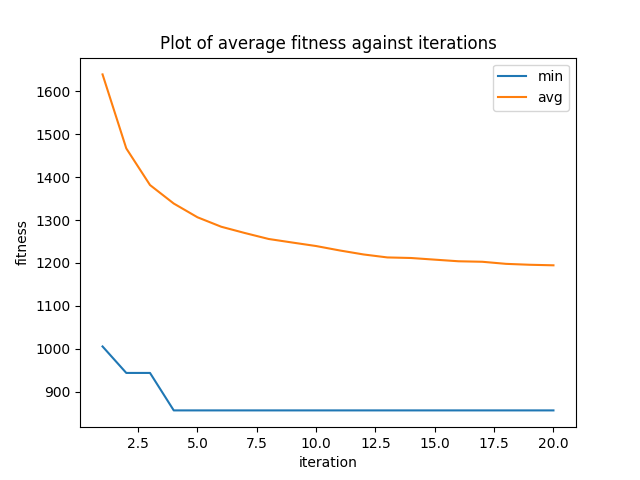
\includegraphics[width=1\linewidth]{images/n32-k5_20.png}
    \caption{ACO with 20 iterations}
    \label{fig:n32-k5_20}
  \end{subfigure}%
  \begin{subfigure}{.5\textwidth}
    \centering
    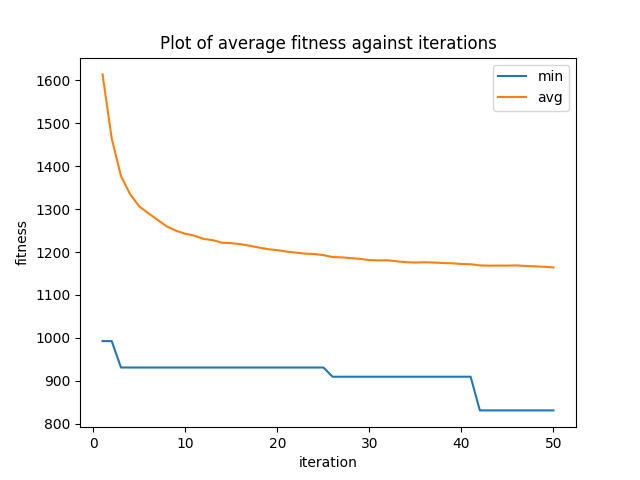
\includegraphics[width=1\linewidth]{images/n32-k5_50.png}
    \caption{ACO with 50 iterations}
    \label{fig:n32-k5_50}
  \end{subfigure}
  \caption{Note: Fitness is the distance}
  \label{fig:n32-k5}
\end{figure}

\begin{figure}[H]
  \centering
  \textbf{Dataset A-n44-k6}
  \begin{subfigure}{.5\textwidth}
    \centering
    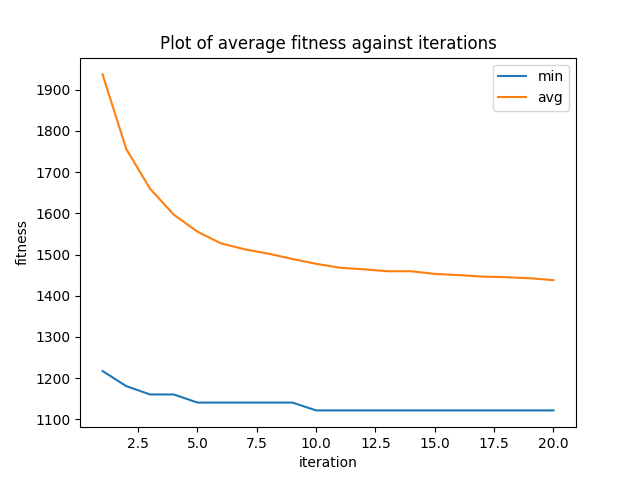
\includegraphics[width=1\linewidth]{images/n44-k6_20.png}
    \caption{ACO with 20 iterations}
    \label{fig:n44-k6_20}
  \end{subfigure}%
  \begin{subfigure}{.5\textwidth}
    \centering
    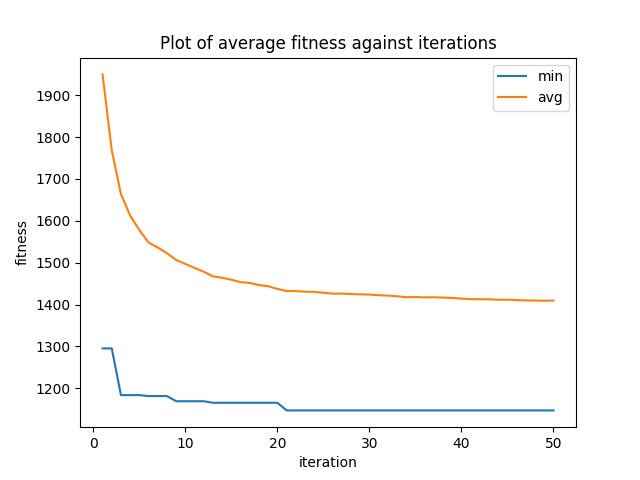
\includegraphics[width=1\linewidth]{images/n44-k6_50.png}
    \caption{ACO with 50 iterations}
    \label{fig:n44-k6_50}
  \end{subfigure}
  \caption{Note: Fitness is the distance}
  \label{fig:n44-k6}
\end{figure}

\begin{figure}[H]
  \centering
  \textbf{Dataset A-n60-k9}
  \begin{subfigure}{.5\textwidth}
    \centering
    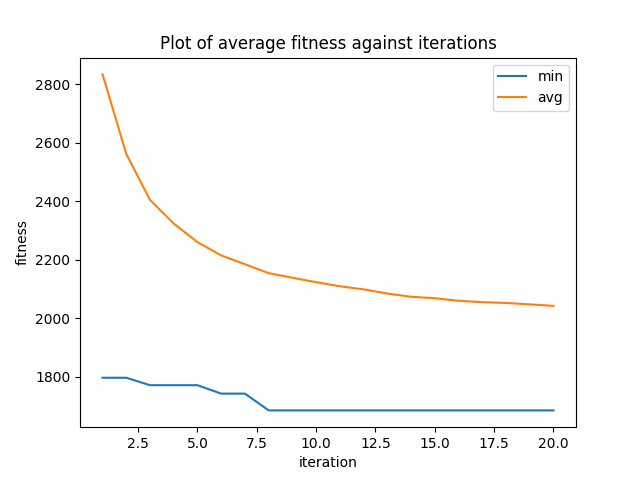
\includegraphics[width=1\linewidth]{images/n60-k9_20.png}
    \caption{ACO with 20 iterations}
    \label{fig:n60-k9_20}
  \end{subfigure}%
  \begin{subfigure}{.5\textwidth}
    \centering
    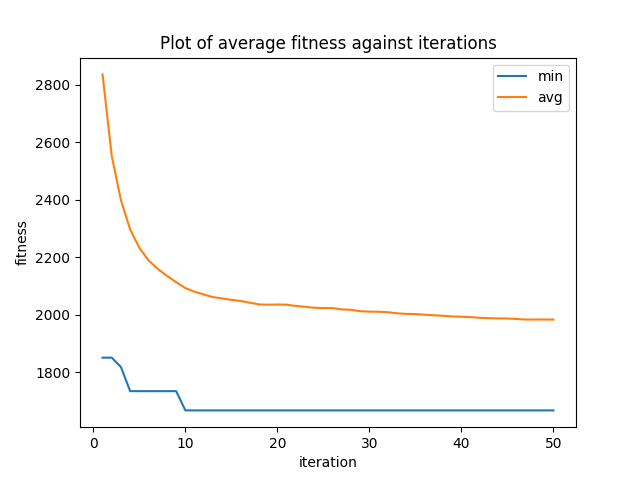
\includegraphics[width=1\linewidth]{images/n60-k9_50.png}
    \caption{ACO with 50 iterations}
    \label{fig:n60-k9_50}
  \end{subfigure}
  \caption{Note: Fitness is the distance}
  \label{fig:60-k9}
\end{figure}

\begin{figure}[H]
  \centering
  \textbf{Dataset A-n80-k10}
  \begin{subfigure}{.5\textwidth}
    \centering
    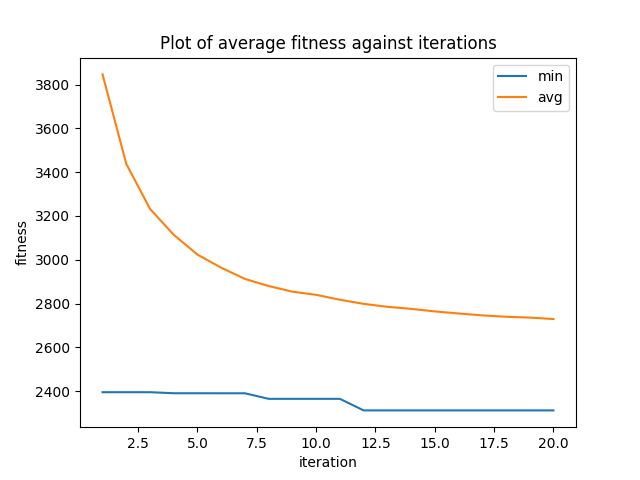
\includegraphics[width=1\linewidth]{images/n80-k10_20.png}
    \caption{ACO with 20 iterations}
    \label{fig:n80-k10_20}
  \end{subfigure}%
  \begin{subfigure}{.5\textwidth}
    \centering
    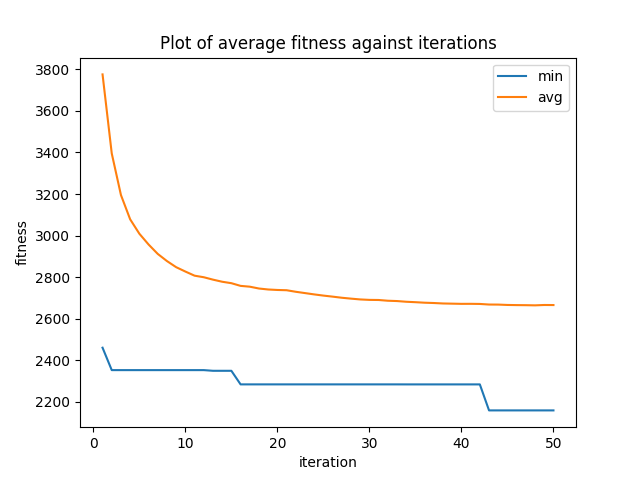
\includegraphics[width=1\linewidth]{images/n80-k10_50.png}
    \caption{ACO with 50 iterations}
    \label{fig:n80-k10_50}
  \end{subfigure}
  \caption{Note: Fitness is the distance}
  \label{fig:n80-k10}
\end{figure}

\end{document}